\documentclass[20pt]{extarticle}

% Généralités
\usepackage[french]{babel}
\usepackage[utf8]{inputenc}
\usepackage{lmodern}
\usepackage[T1]{fontenc}
\usepackage[margin=2cm, headsep=0cm, headheight=25pt]{geometry}
\usepackage{hyperref}
\usepackage{caption}

% Police
% \renewcommand{\familydefault}{\sfdefault}
% \usepackage{cmbright}
% %\usepackage[math]{iwona}

% Tikz
\usepackage{tikz}
\usetikzlibrary{decorations.pathreplacing}

% Maths
\usepackage{amssymb}
\usepackage{amsmath}

% Spécifiques document
\newcommand{\lc}[1]{l_{#1}}
\newcommand{\neurone}[2]{n_{ #1 }^{ (#2) }}
\newcommand{\poids}[3]{p_{#1, #2}^{ (#3) }}
\newcommand{\nps}[2]{\sigma_{ #1 }^{ (#2) }} % "neurone produit scalaire"
\newcommand{\err}[3]{e_{ #1 #2 }^{ (#3) }}
\newcommand{\er}[2]{e_{ #1}^{ (#2) }} % notation simplifiée

% En têtes, pieds de page
\usepackage{fancyhdr}
\lhead{}
\chead{}
\rhead{\color{gris} \textbf{Reconnaissance de caractères}}
\lfoot{}
\cfoot{}
\rfoot{}
\renewcommand{\headrulewidth}{0pt}
\renewcommand{\footrulewidth}{0pt}

% Listes
\usepackage{enumitem}
\frenchbsetup{StandardItemizeEnv=true, StandardEnumerateEnv=true}
\setlist[itemize]{label=$\triangleright$, itemsep=0.5cm}

% Couleurs
\usepackage{xcolor}
\definecolor{gris}{gray}{0.2}

% Pour des bouts de code
\usepackage{listings}
\lstset{
  basicstyle=\ttfamily\small, 
  keywordstyle=\textbf,
  commentstyle=\color{gris},
  stringstyle=\textit,
  showstringspaces=false,
  tabsize=2,
  breaklines=true
}

% Émulations diaporama
\newenvironment{slide}{\topskip 0pt \vspace*{\fill}}{\vspace*{\fill}}
\newcommand{\slidetitle}[1]{\hfill \textbf{\large #1}}

% Autres
\newcommand{\coderef}[1]{\raisebox{10pt}{{\scriptsize \texttt{[#1]}}}}

\begin{document}

% \pagestyle{empty}

% \begin{slide}

% 	\begin{center}

% 		\textbf{\color{gris} \Huge OCR} \\ 
% 		\vspace{0.5cm} 
% 		\textbf{\color{gris} \Large Reconnaissance de caractères} \\
% 		\vspace{1cm}
% 		Brondeau Victor, Nédélec Silvère, Trendel Alexandre \\

% 		\vspace{8cm}
% 		\textbf{\small \color{gris} TIPE session 2016 \\ \flqq{} Structures : organisation, complexité, dynamique. \frqq{}}

% 	\end{center}

% \end{slide}

\clearpage
\pagestyle{fancy}
\slidetitle{Principe général}

\begin{slide}

\begin{itemize}

	\item \textbf{Traitement d'images:}
	\begin{enumerate}
		\item conversion en noir et blanc;
		\item retrait des parasites éventuels;
		\item séparation des caractères; 
		\item conversion en vecteur.
	\end{enumerate}

	\item \textbf{Reconnaissance des caractères:} utilisation d'un \textit{réseau de neurones artificiels} et d'un algorithme d'apprentissage supervisé.

\end{itemize}
	
\end{slide}
\clearpage
\slidetitle{Conversion en vecteur}

\begin{slide} 

\begin{itemize}

	\item On peut se contenter d'aplanir la matrice des pixels de l'image, mais vecteur trop grand.
	
	\item \textbf{Autre méthode:} placer une grille sur l'image, calculer la \textit{proportion} de pixels noirs dans chaque zone, aplanir la nouvelle matrice obtenue.

\end{itemize}	

\begin{figure}[h!]
	\centering
	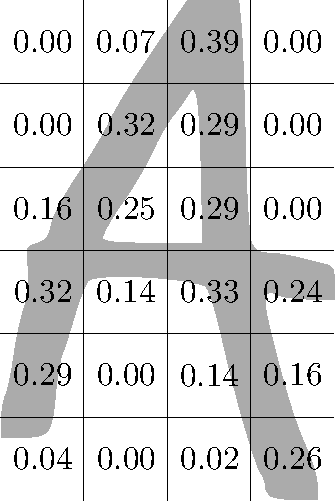
\includegraphics[width=6cm]{schemas/vectorisation.pdf}
\end{figure}

\end{slide}
\clearpage
\slidetitle{Réseaux et neurones}

\begin{slide}

\begin{itemize}

	\item \textbf{Neurone:} associe à un vecteur $x = (x_1, \ldots, x_m)$ une sortie scalaire $\varphi(x)$, entrées pondérées par un \textit{poids} $p_i$ puis composition par une \textit{fonction d'activation} $f$ translatée par un \textit{biais} $b$.
	\begin{equation*}
		\varphi(x) = f (\sum_{i=1}^m p_i x_i - b) 
	\end{equation*}

	\item Fonction d'activation usuelle : $f(x) = \frac{1}{1 + \mathrm{e}^{-x}}$.

	\begin{figure}[h!]
	\centering
	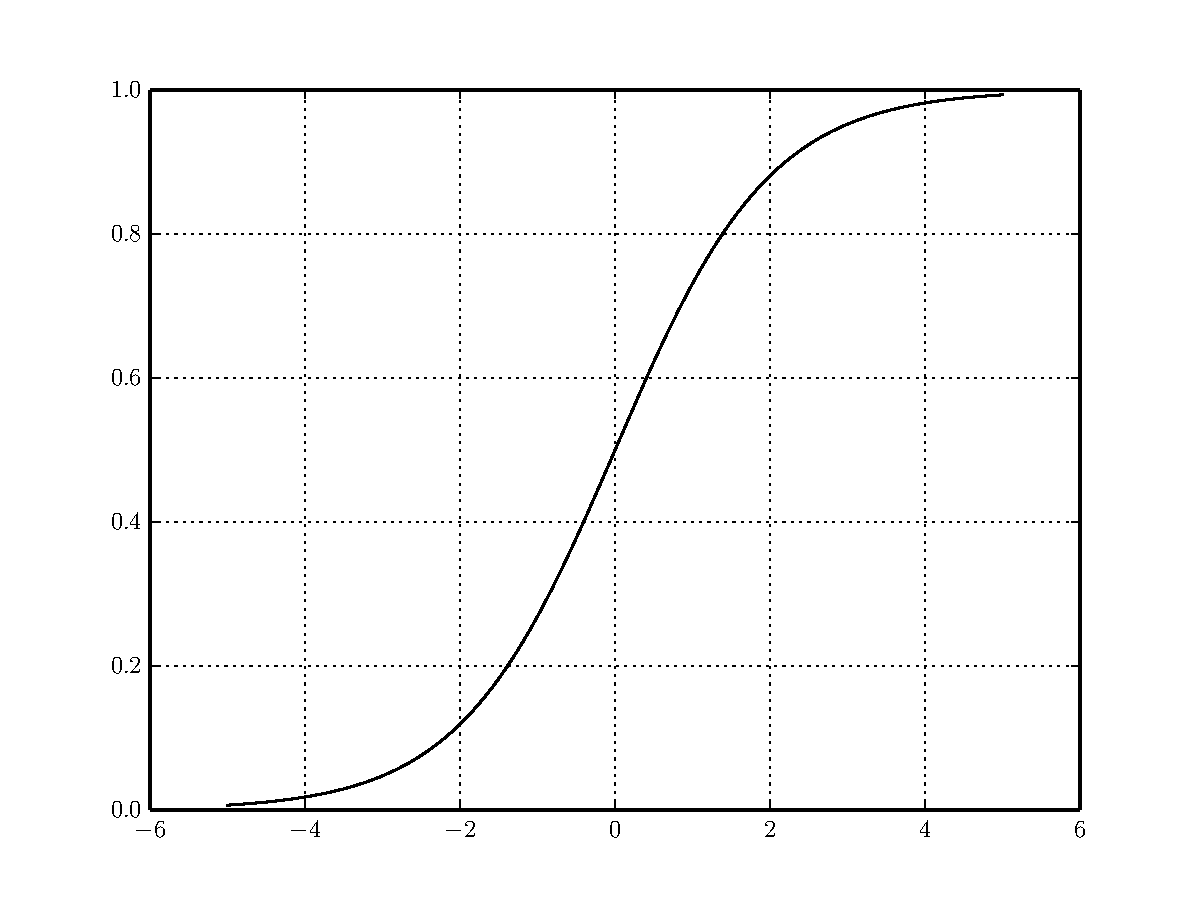
\includegraphics[width=0.8\linewidth]{schemas/sigmoide.pdf}
	\end{figure}

\end{itemize}

\end{slide}

\clearpage
\slidetitle{Réseaux et neurones}

\begin{slide}

\begin{itemize}

	\item \textbf{Réseau:} application de $\mathbb{R}^p$ dans $\mathbb{R}^q$, modélisée par des couches de neurones.

	\item \textbf{Organisation en couches:} l'ensemble des sorties scalaires des neurones de la couche $c$ notées $\neurone{i}{c}$ sert d'entrée aux neurones de la couche $c+1$:
	\begin{equation*}
		\neurone{j}{c+1} = f ( \sum_{i=1}^{\lc{c}} \poids{i}{j}{c+1} \neurone{i}{c} ) = f( \nps{j}{c+1} ).
	\end{equation*}

\end{itemize}

\begin{figure}[!h]

	\centering

	\begin{tikzpicture}[font=\normalsize, scale=0.8, x=1cm, y=1cm]

		\tikzstyle{neurone}=[draw, transform shape, circle, minimum size=3cm]
		\tikzstyle{fleche}=[->, >=latex]
		\tikzstyle{gris}=[dashed, gray]
		\tikzstyle{poids}=[midway, sloped, above]

		\node[neurone] (x1) at (0, 13) {$\neurone{1}{c}$};
		\node[neurone] (x2) at (0, 9) {$\neurone{2}{c}$};
		\draw (0, 6.5) node {\vdots};
		\node[neurone] (xk) at (0, 4) {$\neurone{\lc{c}-1}{c}$};
		\node[neurone] (biais) at (0, 0) {-1};
		\node[neurone] (xj) at (8, 8.5) {$\neurone{j}{c+1}$};
		\node[neurone, gris] (xj+1) at (8, 4.4) {$\neurone{j+1}{c+1}$};

		\draw[fleche, gris] (x1) -- (xj+1) node[poids] {};
		\draw[fleche, gris] (x2) -- (xj+1) node[poids] {};
		\draw[fleche, gris] (xk) -- (xj+1) node[poids] {};
		\draw[fleche, gris] (biais) -- (xj+1) node[poids] {};
		\draw[fleche] (x1) -- (xj) node[poids] {$\poids{1}{j}{c+1}$};
		\draw[fleche] (x2) -- (xj) node[poids] {$\poids{2}{j}{c+1}$};
		\draw[fleche] (xk) -- (xj) node[poids] {$\poids{\lc{c}-1}{j}{c+1}$};
		\draw[fleche] (biais) -- (xj) node[poids] {$\poids{\lc{c}}{j}{c+1}$};

	\end{tikzpicture}

\end{figure}

\end{slide}
\clearpage
\slidetitle{Reconnaissance}

\begin{slide}

\begin{itemize}

	\item On choisit une association entre vecteur de sortie dans $\mathbb{R}^q$ et caractères à reconnaître:

	\begin{equation*}
		\begin{pmatrix}
			1 \\ 0 \\ 0 \\ \vdots \\ 0
		\end{pmatrix}
		\mapsto \text{"A"}
		\qquad
		\begin{pmatrix}
			0 \\ 1 \\ 0 \\ \vdots \\ 0
		\end{pmatrix}
		\mapsto \text{"B"}.
	\end{equation*}


	\item Si les poids sont adaptés, le principe de reconnaissance est simple.

% 	\item Calcul récursif de l'image \texttt{sorties[-1]} du \texttt{Reseau}.

% \begin{lstlisting}[language=Python]
% def sortie(self, vecteur):
% 	sorties = [vecteur + [-1]]
% 	taille = len(self)
% 	for couche in self:
% 		sortie = [neurone.sortie(sorties[-1]) for neurone in couche] 
% 		if len(sorties) < taille:
% 			sortie += [-1]
% 		sorties.append(sortie)
% 	return sorties
% \end{lstlisting}

\end{itemize}

\begin{figure}[!h]

	\centering

	\begin{tikzpicture}[scale=1, x=1cm, y=1cm]

		\tikzstyle{neurone}=[draw, transform shape, circle, minimum size=2cm]
		\tikzstyle{entree}=[draw, transform shape, rectangle, minimum size=1.5cm]
		\tikzstyle{fleche}=[->, >=latex, gray]

		\node at (-1, 0) {
		$\begin{pmatrix}
			0.00 \\ 0.07 \\ 0.39 \\ 0.00 \\ \vdots \\ 0.02 \\ 0.26
		\end{pmatrix}$
		};

		\node (e1) at (0, -2) {};
		\node (e2) at (0, 0) {};
		\node (e3) at (0, 2) {};

		\node[neurone] (n11) at (4, 3.75) {};
		\node[neurone] (n12) at (4, 1.25) {};
		\node[neurone] (n13) at (4, -1.25) {};
		\node[neurone] (n14) at (4, -3.75) {};

		\node[neurone] (n21) at (8, 2.5) {};
		\node[neurone] (n22) at (8, 0) {};
		\node[neurone] (n23) at (8, -2.5) {};

		\draw[fleche] (e1) -- (n11);
		\draw[fleche] (e1) -- (n12);
		\draw[fleche] (e1) -- (n13);
		\draw[fleche] (e1) -- (n14);
		\draw[fleche] (e2) -- (n11);
		\draw[fleche] (e2) -- (n12);
		\draw[fleche] (e2) -- (n13);
		\draw[fleche] (e2) -- (n14);
		\draw[fleche] (e3) -- (n11);
		\draw[fleche] (e3) -- (n12);
		\draw[fleche] (e3) -- (n13);
		\draw[fleche] (e3) -- (n14);

		\draw[fleche] (n11) -- (n21);
		\draw[fleche] (n11) -- (n22);
		\draw[fleche] (n11) -- (n23);
		\draw[fleche] (n12) -- (n21);
		\draw[fleche] (n12) -- (n22);
		\draw[fleche] (n12) -- (n23);
		\draw[fleche] (n13) -- (n21);
		\draw[fleche] (n13) -- (n22);
		\draw[fleche] (n13) -- (n23);
		\draw[fleche] (n14) -- (n21);
		\draw[fleche] (n14) -- (n22);
		\draw[fleche] (n14) -- (n23);

		\node (s1) at (11, 2.5) {$0.91$};
		\node (s2) at (11, 0) {$0.12$};
		\node (s3) at (11, -2.5) {$0.08$};

		\draw[fleche] (n21) -- (s1);
		\draw[fleche] (n22) -- (s2);
		\draw[fleche] (n23) -- (s3);

		% \draw[thick, decoration={brace, amplitude=0.3cm}, decorate] (s1.north east) -- (s3.south east);
		% \node[align=left, xshift=2.5cm] at (s2.east) {comparaison\\ aux vecteurs\\ choisis};

	\end{tikzpicture}

\end{figure}

\end{slide}
\clearpage
\slidetitle{Apprentissage supervisé}

\begin{slide}

\begin{itemize}

	\item Calcul de l'image $y$ par le réseau de quelques échantillons $x$.
	\begin{center}
		
\includegraphics[width=0.075\linewidth]{a/0.png} \quad
		
\includegraphics[width=0.075\linewidth]{a/1.png} \quad
		
\includegraphics[width=0.075\linewidth]{a/2.png} \quad
		
\includegraphics[width=0.075\linewidth]{a/3.png} \quad
		
\includegraphics[width=0.075\linewidth]{a/4.png}
	\end{center}
	
	\item Comparaison de $y$ et de la valeur vectorielle $t$ que l'on souhaite associer aux exemples à l'aide d'une fonction d'erreur:
	\begin{equation*}
		E = \frac{1}{2} \sum_{i=1}^q (t_i - y_i)^2.
	\end{equation*}

	\item Correction des valeurs des poids, modulée par un \textit{taux d'apprentissage} $\alpha$ que l'on fixe au départ:
	\begin{equation*}
		\Delta \poids{j}{k}{c} = - \alpha \frac{\partial E}{\partial \poids{j}{k}{c}}.
	\end{equation*}

	\item On répète ces étapes pour chaque caractère à reconnaître (associé à un unique vecteur $t$).

	\end{itemize}

\end{slide}
\clearpage
\slidetitle{Rétropropagation}

\begin{slide}

\begin{itemize}

	\item Posons pour tout neurone indicé $k$ d'une couche $c$
	\begin{equation*}
		\er{k}{c} = - \frac{ \partial E }{ \partial \poids{j}{k}{c} } \frac{1}{ \neurone{j}{c-1} }.
	\end{equation*}

	\item La correction à apporter à chacun des poids du réseau devient
	\begin{equation*}
		\Delta \poids{j}{k}{c} =  \alpha \er{k}{c} \neurone{j}{c-1}.
	\end{equation*} 

	\item On montre à l'aide de la formule de la chaîne les relations suivantes (réseau à $n$ couches):

	\begin{align*}
		& \er{k}{n} = f'(\nps{k}{n}) (t_k - y_k) \\
		\text{et } & \er{k}{c} = f'(\nps{k}{c}) \sum_{i=1}^{\lc{c+1}} \poids{k}{i}{c+1} \er{i}{c+1}.
	\end{align*}

\end{itemize}

\end{slide}
\clearpage
\slidetitle{Réalisation Python}

\begin{slide}

	\begin{figure}[h]
		\centering
		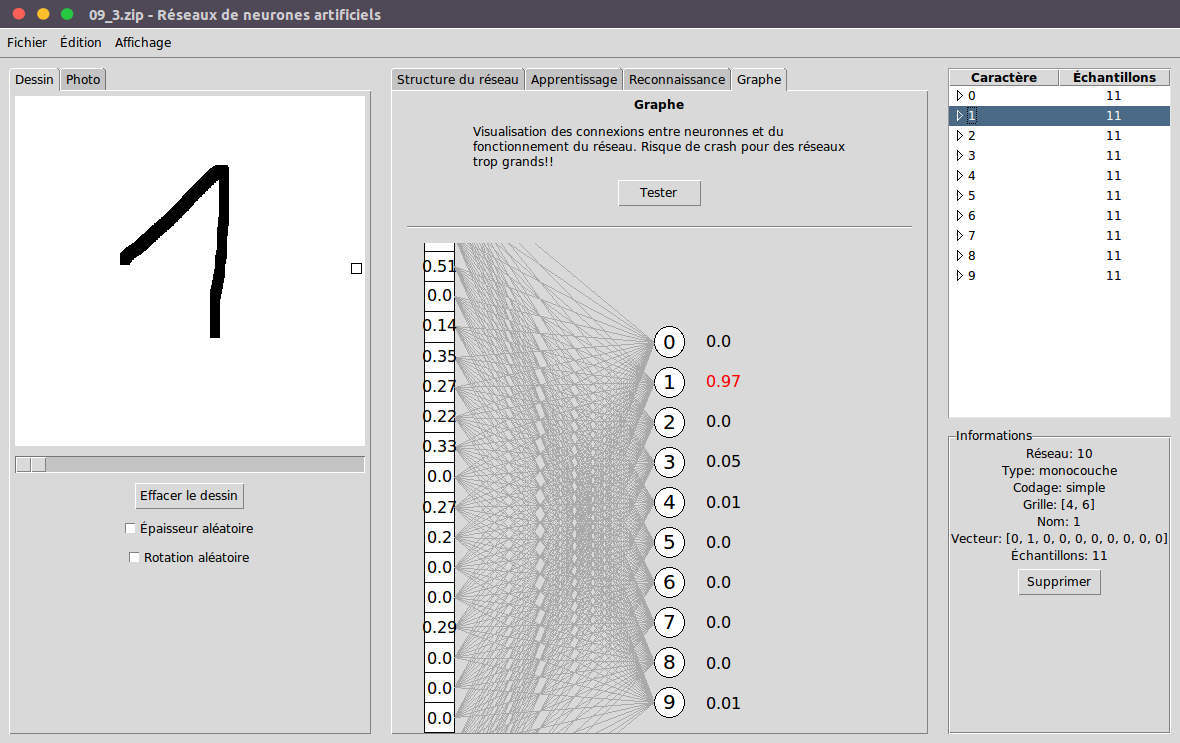
\includegraphics[width=\linewidth]{schemas/capture.png}
	\end{figure}

	\begin{itemize}
		\item Création d'une interface en Python permettant de créer un réseau et de l'entraîner à partir d'échantillons entrés à la souris.
	\end{itemize}

\end{slide}
\clearpage
\slidetitle{Résultats expérimentaux}

\begin{slide}

\begin{itemize}
	\item \textbf{Entrée:} $3\times 5$.
	\item \textbf{Sortie:} chiffres de 0 à 9.
	\item \textbf{Échantillons:} 10 par classe pour l'apprentissage, 1 par classe pour la validation.
\end{itemize}

\begin{figure}[h]
	\centering
	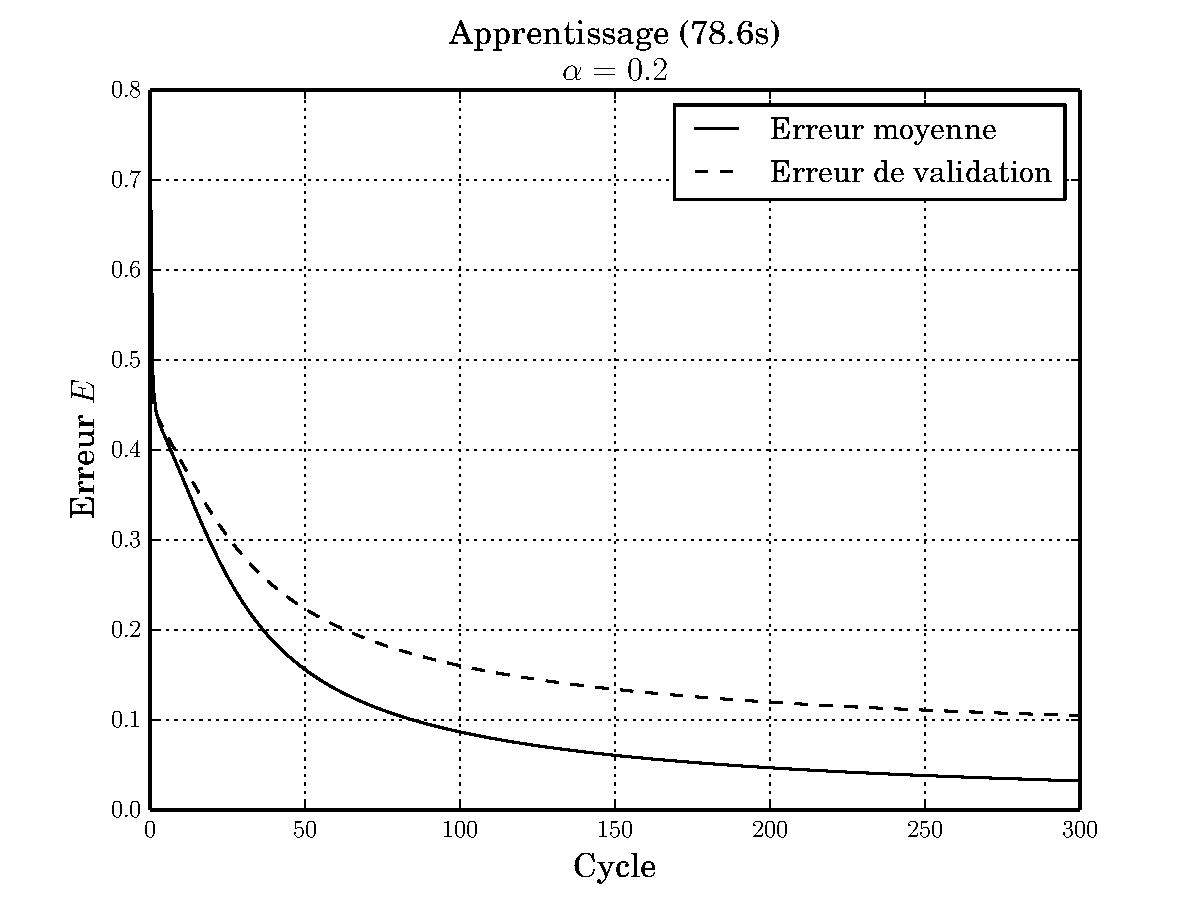
\includegraphics[width=\linewidth]{{graphes/mono_0.2}.pdf}
	\caption*{Monocouche}
\end{figure}

\end{slide}

\clearpage
\slidetitle{Résultats expérimentaux}

\begin{slide}

\begin{figure}[h]
	\centering
	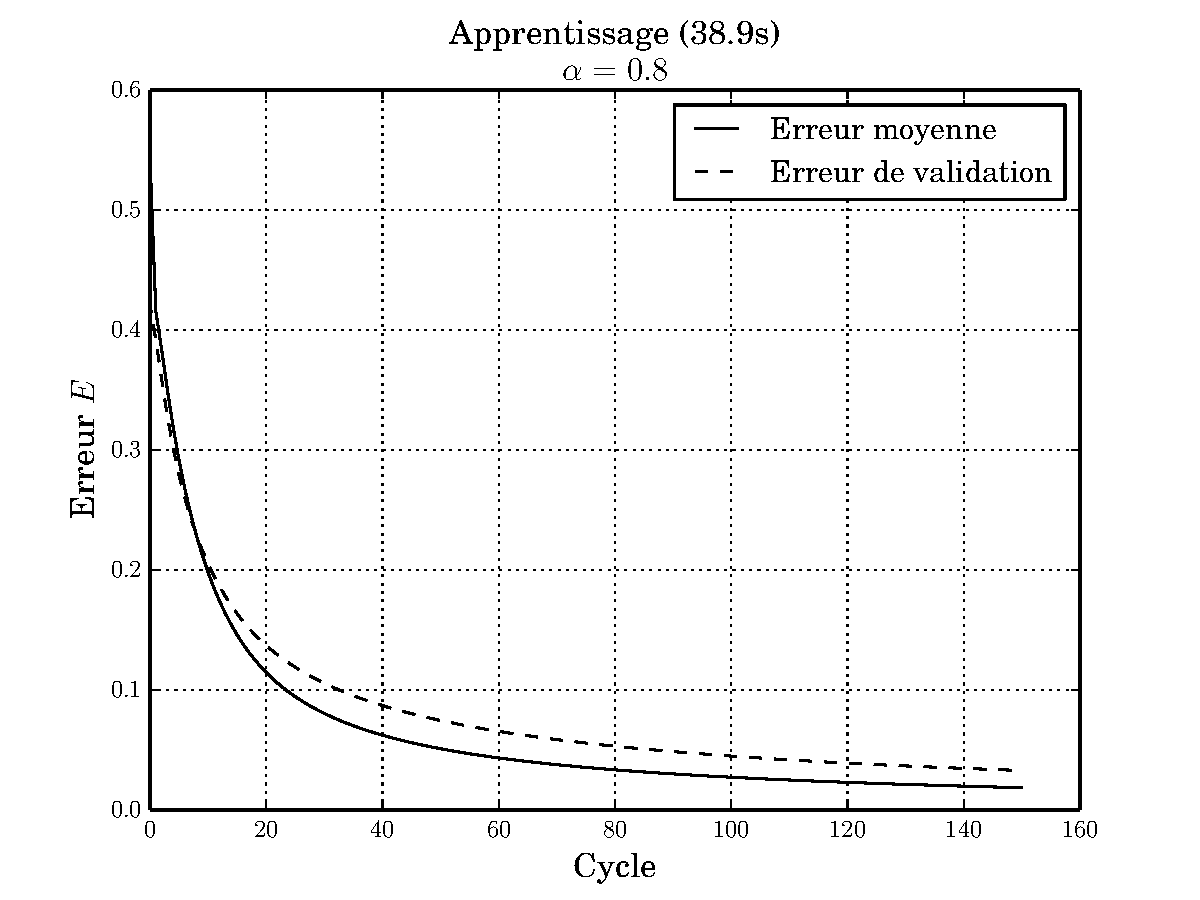
\includegraphics[width=\linewidth]{{graphes/mono_0.8}.pdf}
\end{figure}

\end{slide}

\clearpage
\slidetitle{Résultats expérimentaux}

\begin{slide}

\begin{figure}[h]
	\centering
	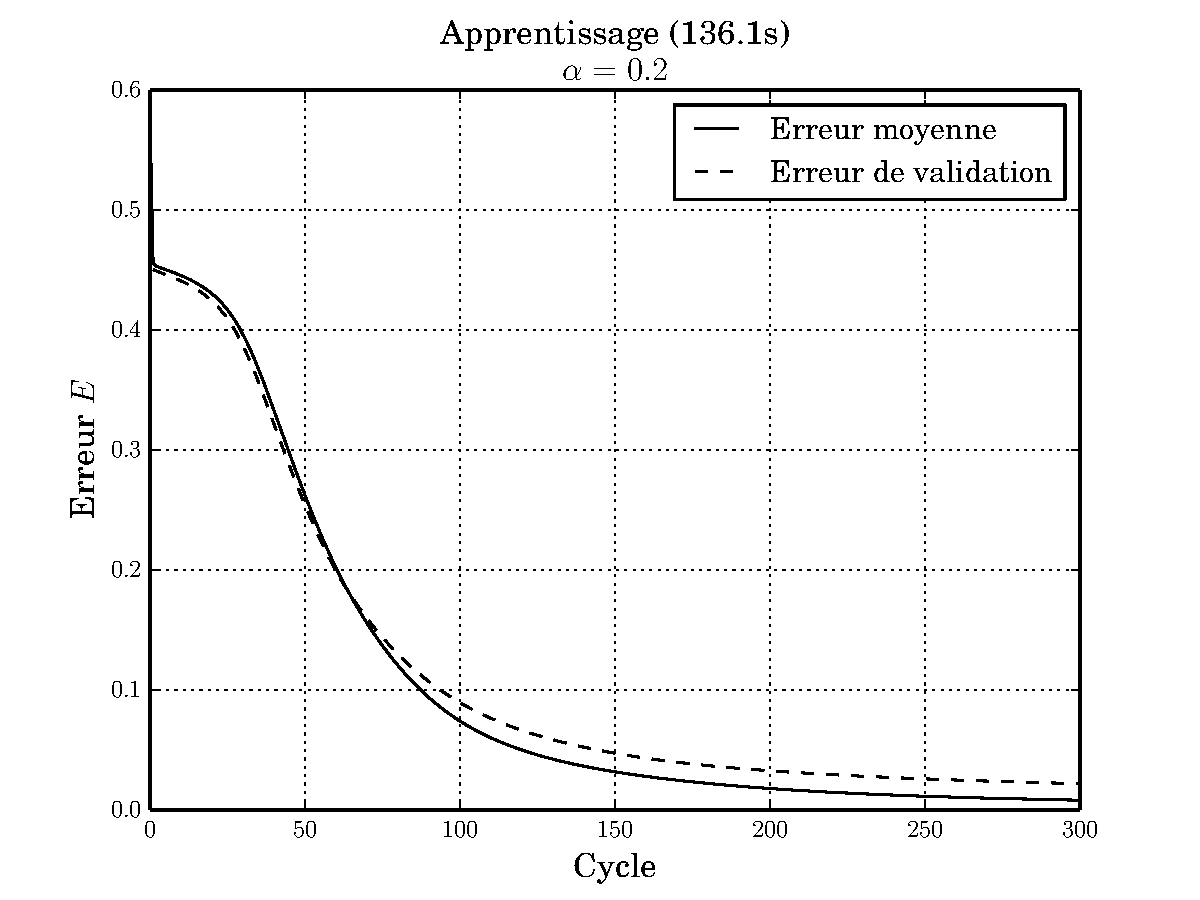
\includegraphics[width=\linewidth]{{graphes/16_0.2}.pdf}
	\caption*{Multicouche (16, 10)}
\end{figure}

\end{slide}

\clearpage
\slidetitle{Résultats expérimentaux}

\begin{slide}

\begin{figure}[h]
	\centering
	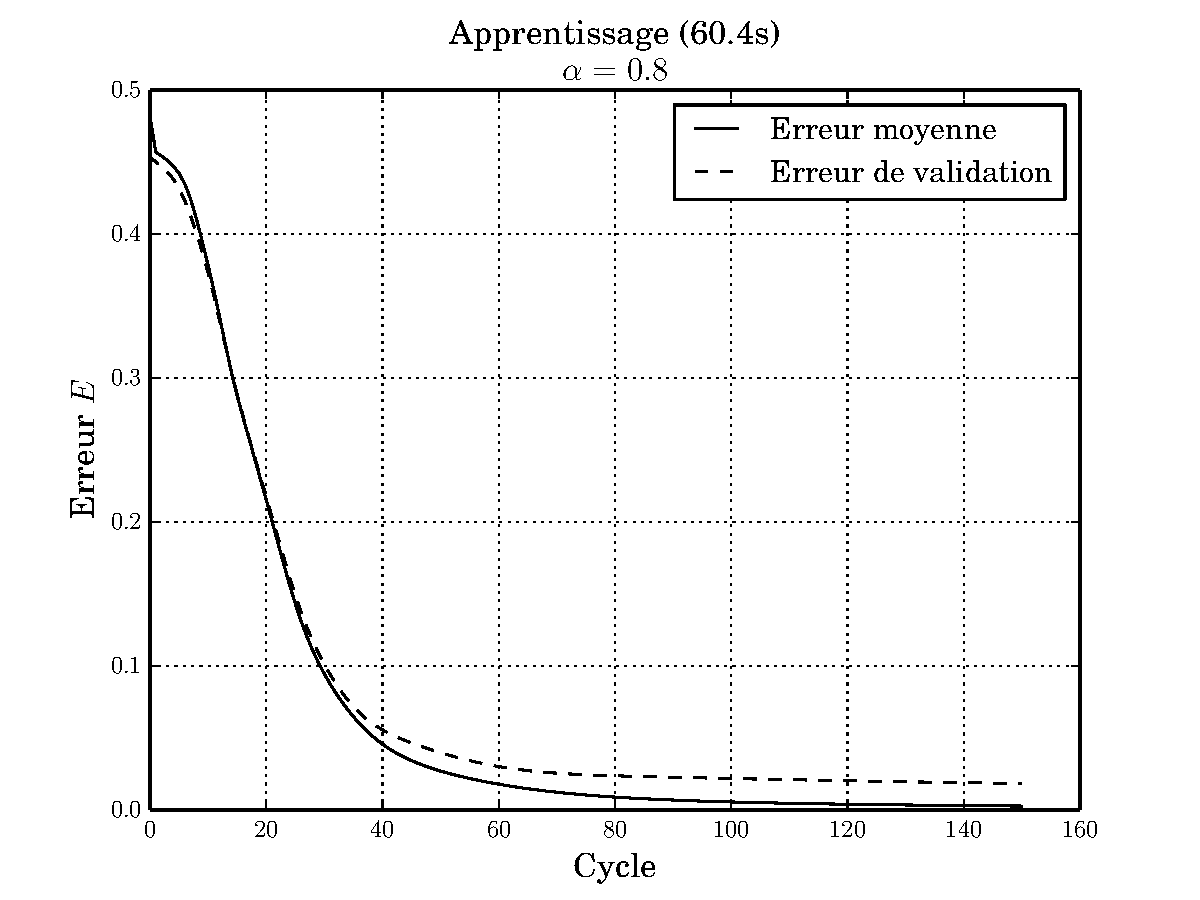
\includegraphics[width=\linewidth]{{graphes/16_0.8}.pdf}
\end{figure}
\end{slide}

\clearpage
\slidetitle{Résultats expérimentaux}

\begin{slide}

\begin{figure}[h]
	\centering
	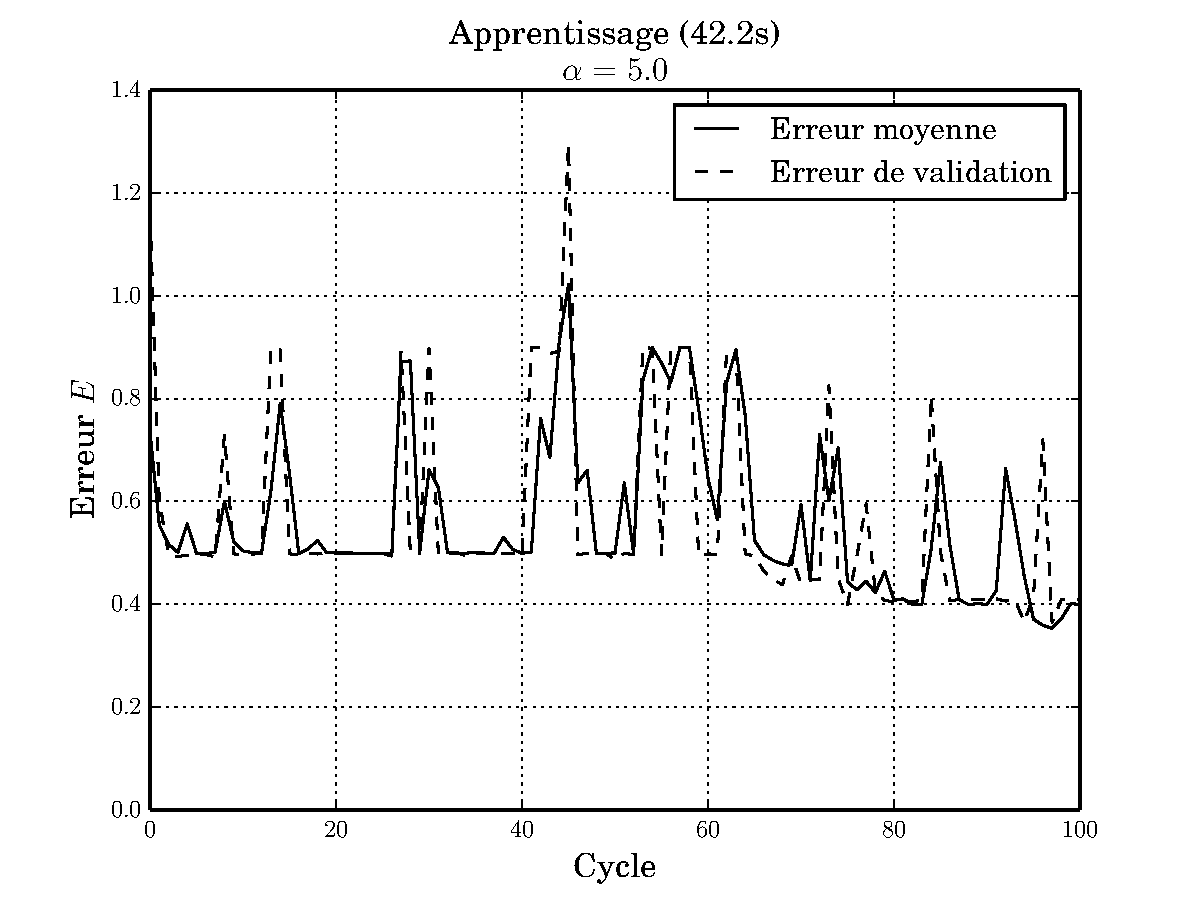
\includegraphics[width=\linewidth]{{graphes/16_5}.pdf}
\end{figure}
\end{slide}

\clearpage
\slidetitle{Résultats expérimentaux}

\begin{slide}

\begin{figure}[h]
	\centering
	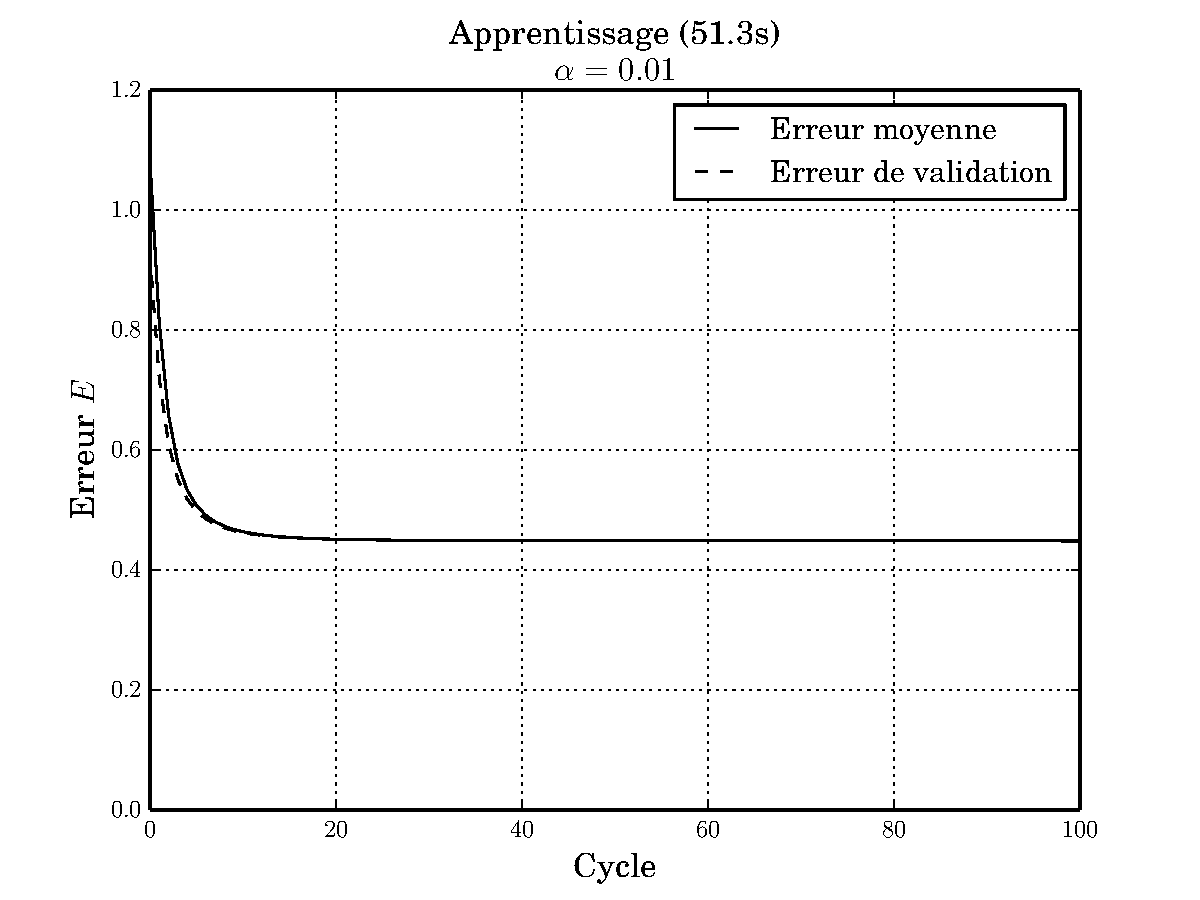
\includegraphics[width=\linewidth]{{graphes/16_12_0.01}.pdf}
	\caption*{Multicouche (16, 12, 10) }
\end{figure}
\end{slide}
%bonus
\clearpage
\slidetitle{Méthode des \textit{k} plus proches voisins}

\begin{slide}

	\begin{itemize}

		\item Alternative très simple aux réseaux de neurones.

		\item On convertit en vecteur l'image du caractère à reconnaître.

		\item L'entier $k$ est fixé. On sélectionne dans la base d'échantillons les $k$ plus proches vecteurs du vecteur image pour la norme euclidienne.

		\item On identifie la classe la plus représentée parmi ces $k$ vecteurs. 

		\item \textbf{Avantage:} pas de phase d'apprentissage, uniquement besoin d'une base d'échantillons.
		\item \textbf{Inconvénient:} il faut avoir une large base d'échantillons accessibles lors de la reconnaissance.

	\end{itemize}

\end{slide}
\clearpage
\slidetitle{Un algorithme de séparation}

\begin{slide}

	\begin{itemize}

		\item Sélection de chaque pixel et de ses pixels adjacents et stockage des groupes temporaires ainsi formés dans une liste $T$.
		\item Initialisation d'une liste (vide) de caractères $C$ (groupes de pixels).
		\item Pour chaque groupe temporaire $a \in T$, et pour chaque caractère $b \in C$, $a$ prend la valeur $a\cup b$ si $a\cap b \neq \emptyset$ et on enlève $b$ de $C$. 
		\item À la fin de la boucle qui parcourt $T$, on ajoute $a$ à $C$, même s'il n'a pas été modifié.

	\end{itemize}

	\begin{figure}[h!]
		\centering
		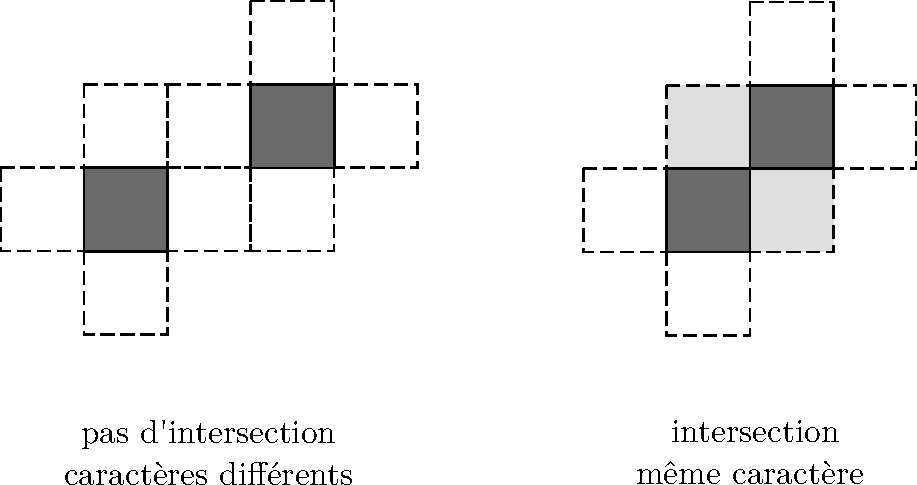
\includegraphics[width=0.8\linewidth]{schemas/algo_sep2.pdf}
	\end{figure}


\end{slide}

\end{document}